\chapter{What is a Genetic Algorithm?}

\begin{figure}
	\centering
		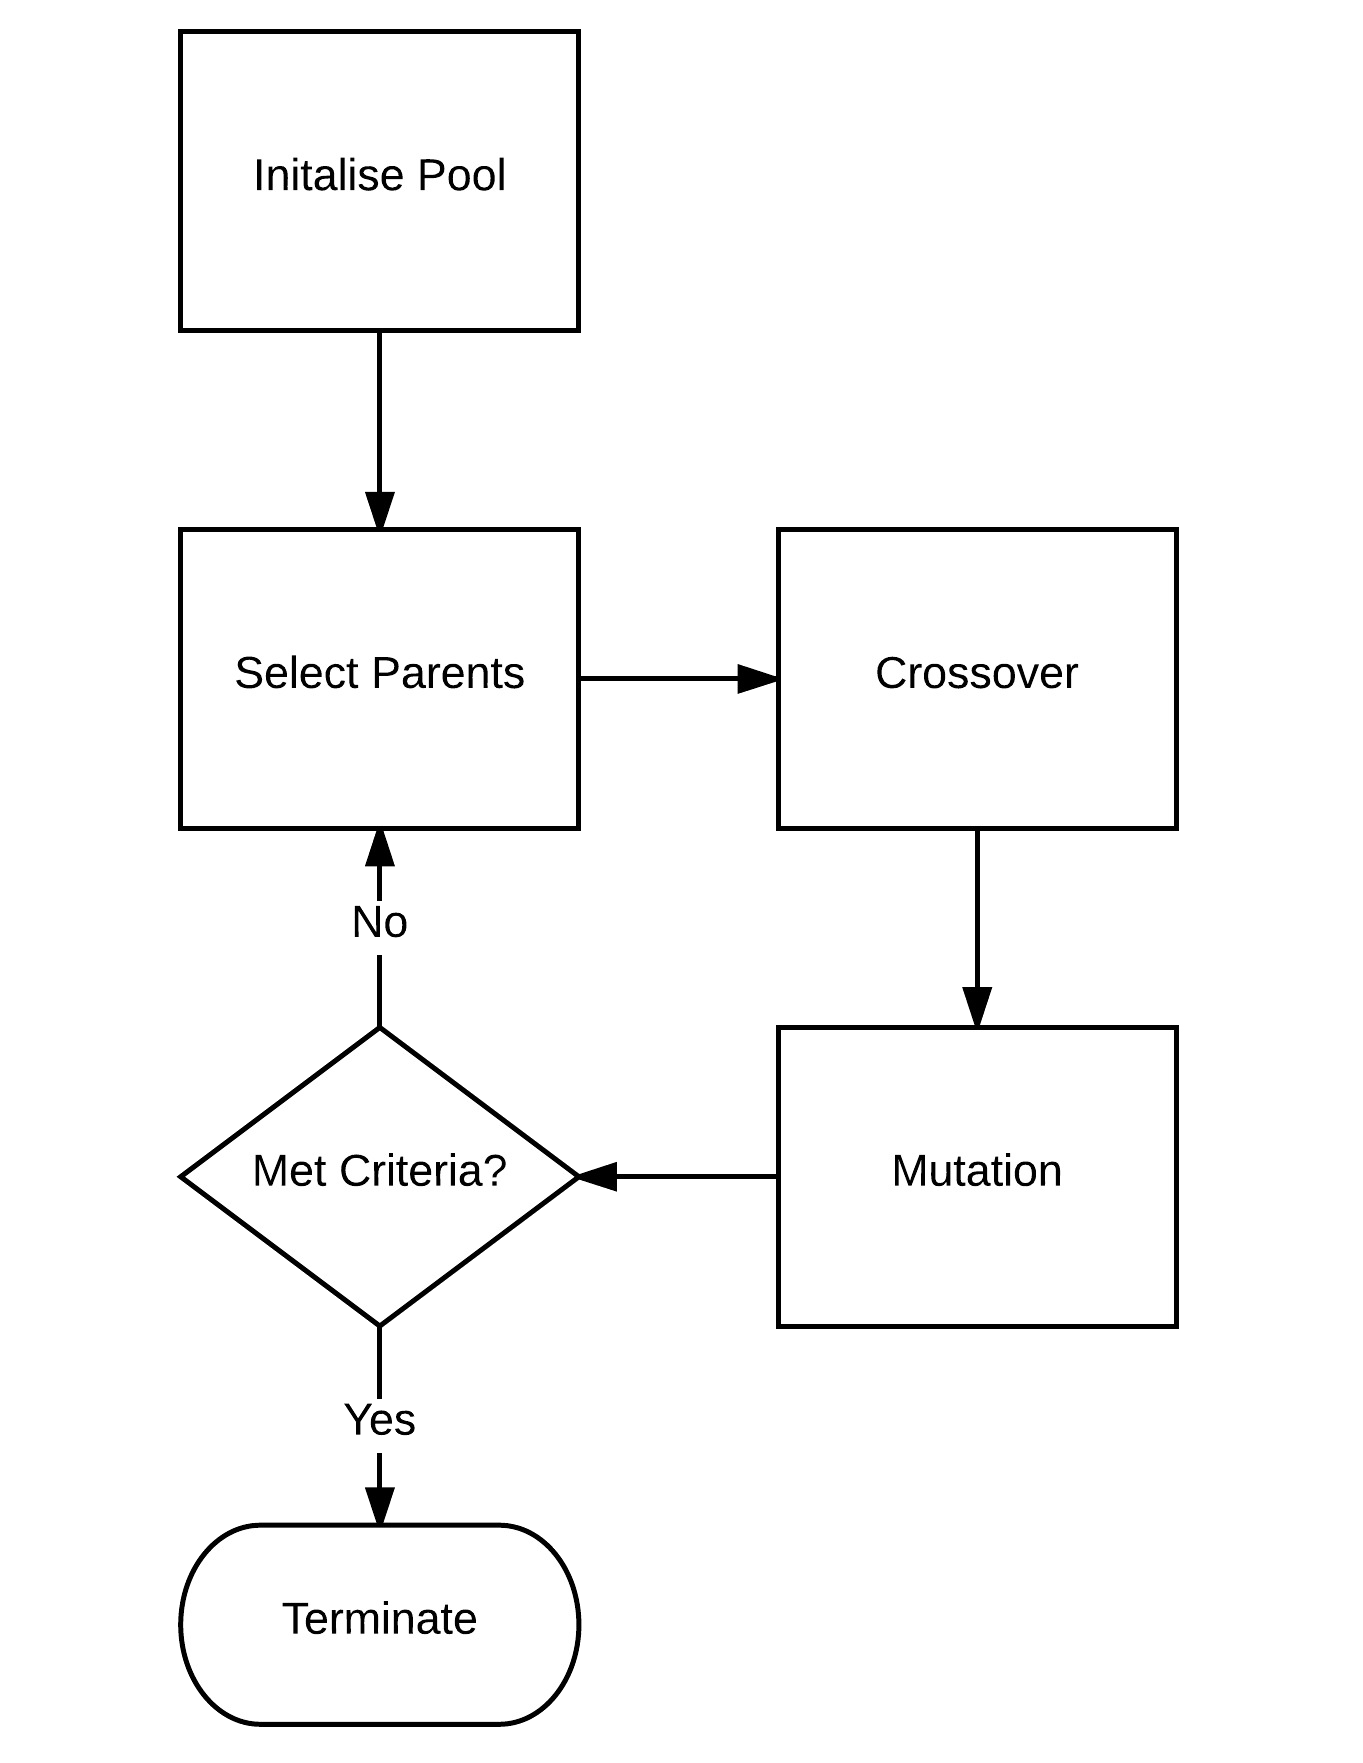
\includegraphics[width=0.5\textwidth]{GA_Structure}
	\caption{The basic structure of a Genetic Algorithm. \label{fig:struct}}

\end{figure}

\par
A Genetic Algorithm is an algorithm that uses natural selection, or survival of the fittest, to find a solution to a problem. All Genetic Algorithms follow a similar, if not identical structure \ref{fig:struct}. However, the elements of said structure are highly customised for each specific application.

\begin{lstlisting}

\end{lstlisting}